\documentclass[aspectratio=169]{beamer}

\usetheme{vega}



\title{}
\subtitle{Влияние макроэкономических показателей страны на уровень индивидуального благополучия граждан}
\author{Заостровский Всеволод, Сулейманов Асхаб, Черепахин Иван}
\supervisor{Станкевич И. П.}
\institute{Vega Institute Foundation, Мехмат МГУ}

\date{}

\usepackage[]{lipsum}
\begin{document}
\maketitle

    

    

\begin{frame}{1.Введение}
\small
   Одним из главных вопросов современной дискуссии является: что же влияет на уровень счастья? Многие убеждены, в том числе и среди видных мыслителей, что счастье в первую очередь зависит от субъективных, мировозренческих, ценностных, идеологических, психологических факторах, нежели чем от объективных факторов по типу благосостояния.

   \begin{figure} \label{hompic}
            \centering
            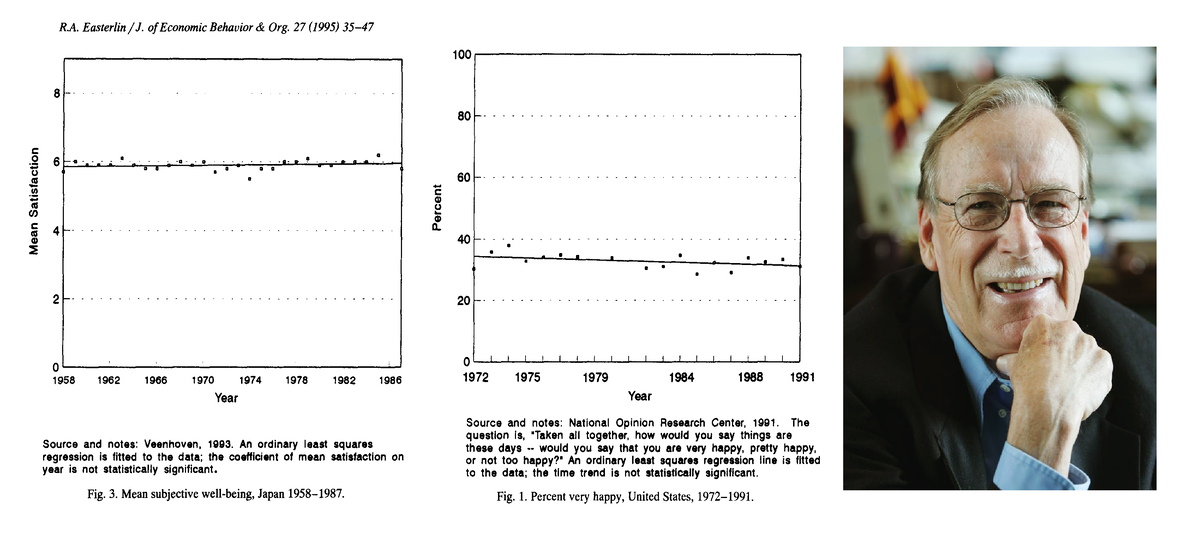
\includegraphics[scale=0.5]{EasterlinU_3_1200x550.png}
    \end{figure}
     
 \end{frame}

\begin{frame}{1.Введение}
\small
    Иные же считают, что главную роль играет не абсолютный уровень богатсва общетсва, а скорее относительный уровень. Например, человек оценивает свою успешность, а соответсвенно и удовлетворенность от жизни, сравнивая себя с другими членами общетства. Приверженцы таких идеи, пытаясь доказать свою правоту, обычно приводят частные примеры, которые, кстати говоря, весьма убедительны и способны склонить колеблющихся в дискуссии в свою сторону. Приведём часть из них, чтоб продемонстрировать всю серьёзность изучаемого вопроса. 

    \begin{figure} \label{hompic}
            \centering
            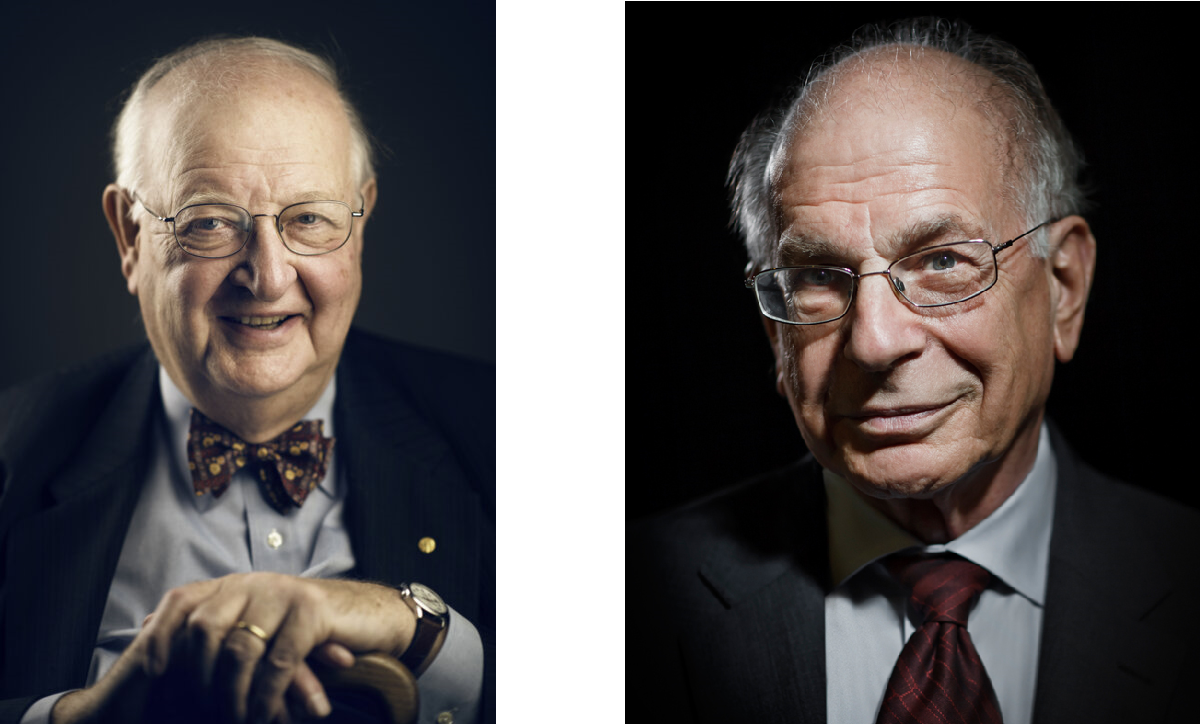
\includegraphics[scale=0.28]{NobleU.png}
    \end{figure}
\end{frame}

\begin{frame}{1.Введение}
\small
   Сообщество World Happiness Report введем постоянный отчет субъективного восприятия людей уровня своего счастья по странам мира. Откуда мы можем получать весьма занимательные факты. Например, такая высокоразвитая страна как Южная Корея, занимающая лидирующие позиции в микроэлектронике, машиностроении, судостроении, атомной энегетике и т.д., по уровню счатья занимает лишь 55 место, на одном уровне с Молдавией, имеющая 100 место по ВВП на душу ППС. Это согласуется и с одним из самых высоких уровней самоубийтсв на душу населения(12 место в мире). И в то же время Узбекистан имеет относительно высокий уровень счастья, занимая 47 место, имея 131 место по ВВП на душу ППС. 
   
   \begin{figure} \label{hompic}
            \centering
            
\includegraphics[scale=0.32]{Union1.png}
    \end{figure}

\end{frame}

\begin{frame}{1.Введение} 
   
   \begin{figure} \label{hompic}
            \centering
            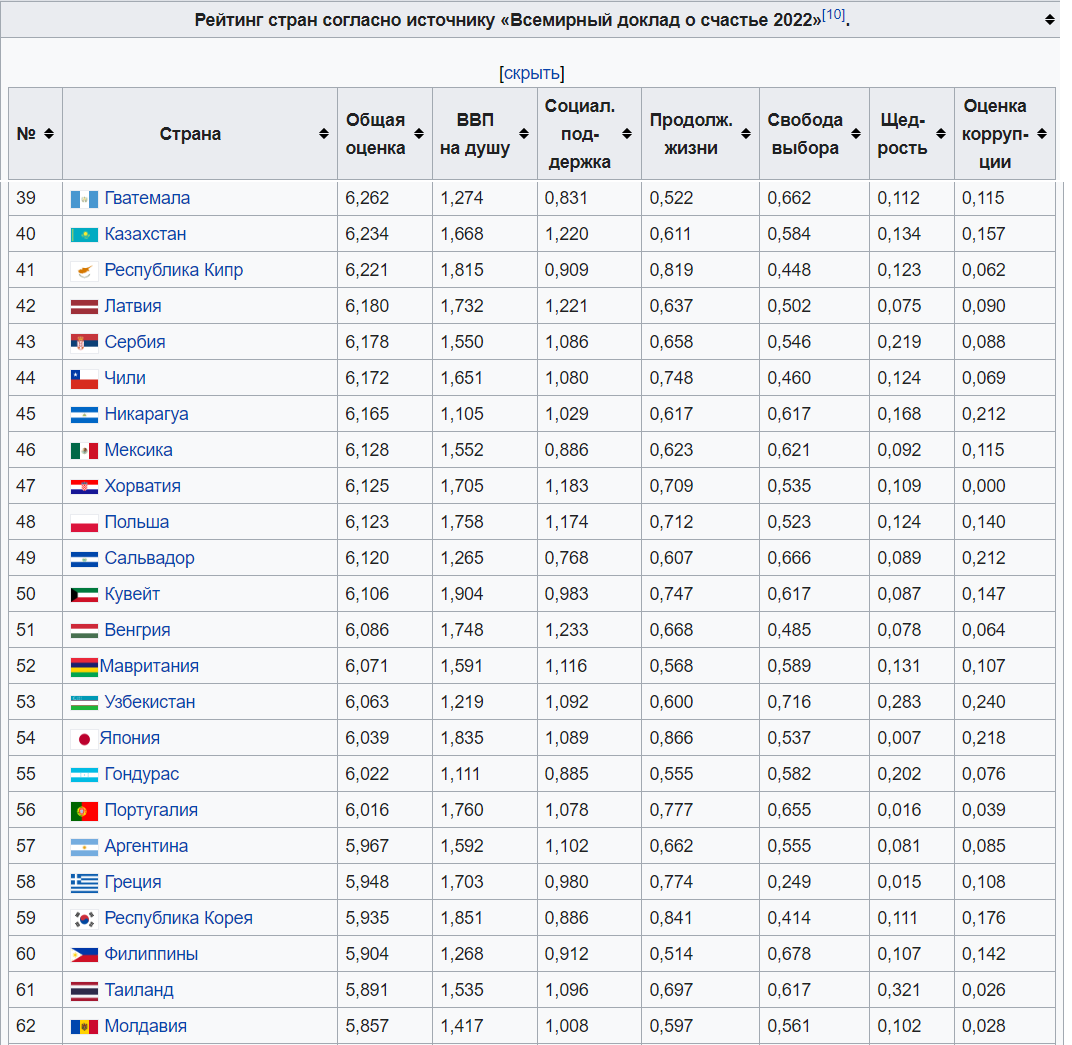
\includegraphics[scale=0.32]{TableKorea.png}
    \end{figure}

\end{frame}

\begin{frame}{1.Введение}
   Мы же попытаемся показать, что макроэкономические достижения стран всё же оказывают существенное влияние на уровень счастья населения хоть и в некоторой усреднённой форме для каждой страны. Мы попытаемся опровергнуть популярный нарратив о незначимости богаства и достижений в качестве жизни для счастья по крайней мере до определенного уровня.  
   \begin{figure} \label{hompic}
            \centering
            
\includegraphics[scale=1]{Union2.png}
    \end{figure}
\end{frame}


\begin{frame}{2.Описание данных. Список данных со ссылками}
В настоящей работе для анализа характеристик стран на макроуровне используются данные Всемирного Банка за 2015-2019 годы. В частности, оттуда была получена следующая информация:


      \item \href{https://data.worldbank.org/indicator/NY.GDP.PCAP.PP.CD}{ВВП по ППС на душу населения.}
        \item \href{https://data.worldbank.org/indicator/GB.XPD.RSDV.GD.ZS?view=chart}{Уровень безработицы.}
        \item \href{https://data.worldbank.org/indicator/IC.TAX.TOTL.CP.ZS?view=chart}{Налоговая нагрузка физических лиц.}
        \item \href{https://data.worldbank.org/indicator/FP.CPI.TOTL.ZG?view=chart}{Инфляция.}
        \item \href{https://data.worldbank.org/indicator/SH.XPD.CHEX.GD.ZS}{Государственные расходы на медицину.}
        \item \href{https://data.worldbank.org/indicator/SE.XPD.TOTL.GD.ZS?view=chart }{Государственные расходы на образование.}
        \item \href{https://data.worldbank.org/indicator/MS.MIL.XPND.GD.ZS}{Государственные военные расходы.}
        \item \href{https://data.worldbank.org/indicator/NY.GNS.ICTR.ZS?view=chart}{Валовая экономия.}
        \item \href{https://data.worldbank.org/indicator/SP.POP.DPND}{Демографическая нагрузка.}
        \item \href{https://data.worldbank.org/indicator/VC.IHR.PSRC.P5}{Число убийств на тысячу человек.}
        
\end{frame}



\begin{frame}{2.Описание данных. Всемирный Банк}
\begin{figure} \label{hompic}
            \centering
            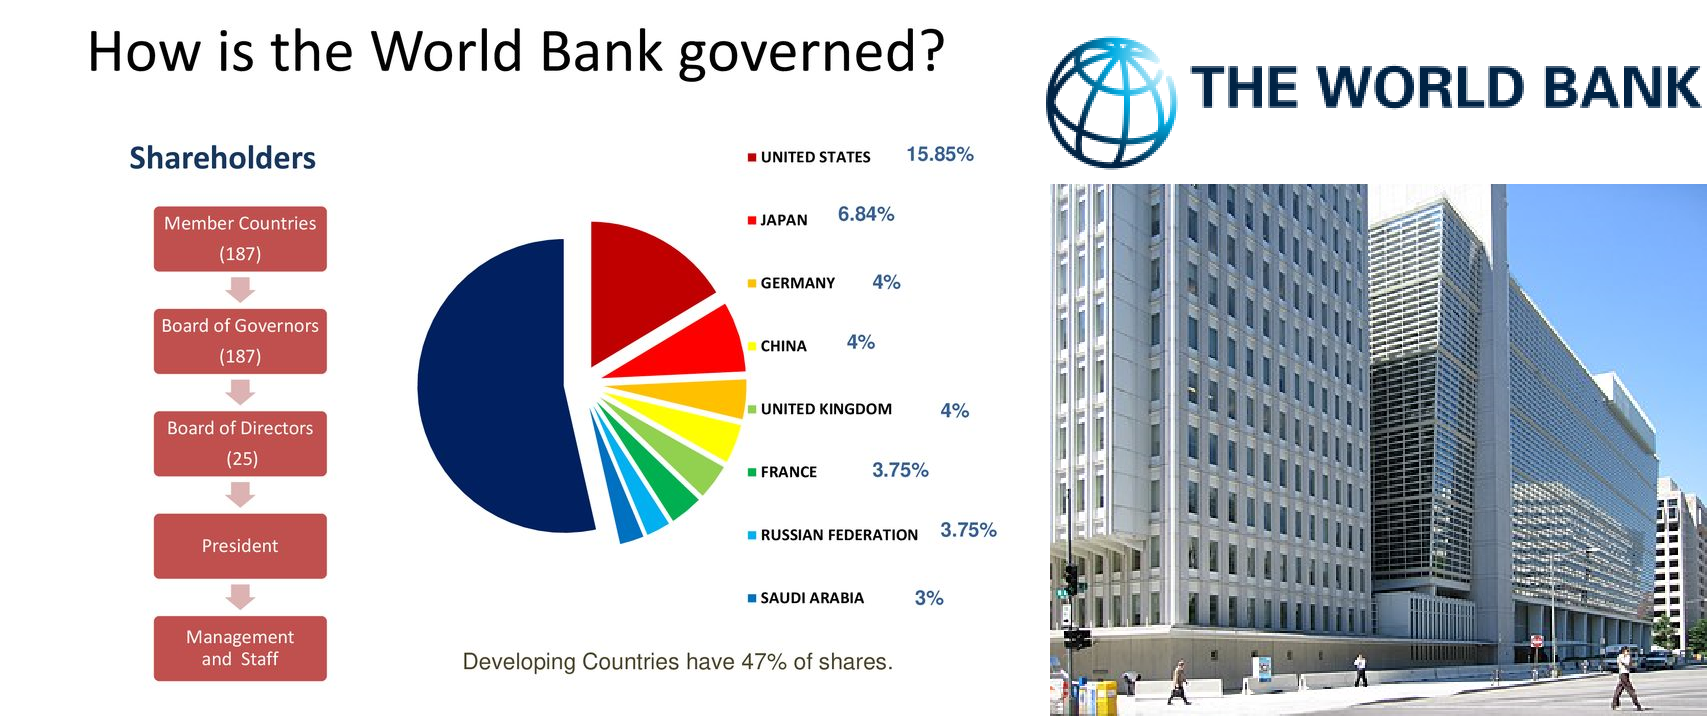
\includegraphics[scale=0.4]{Union4.png}
    \end{figure}
\end{frame}

\begin{frame}{2.Описание данных. Всемирный Банк}
\begin{figure} \label{hompic}
            \centering
            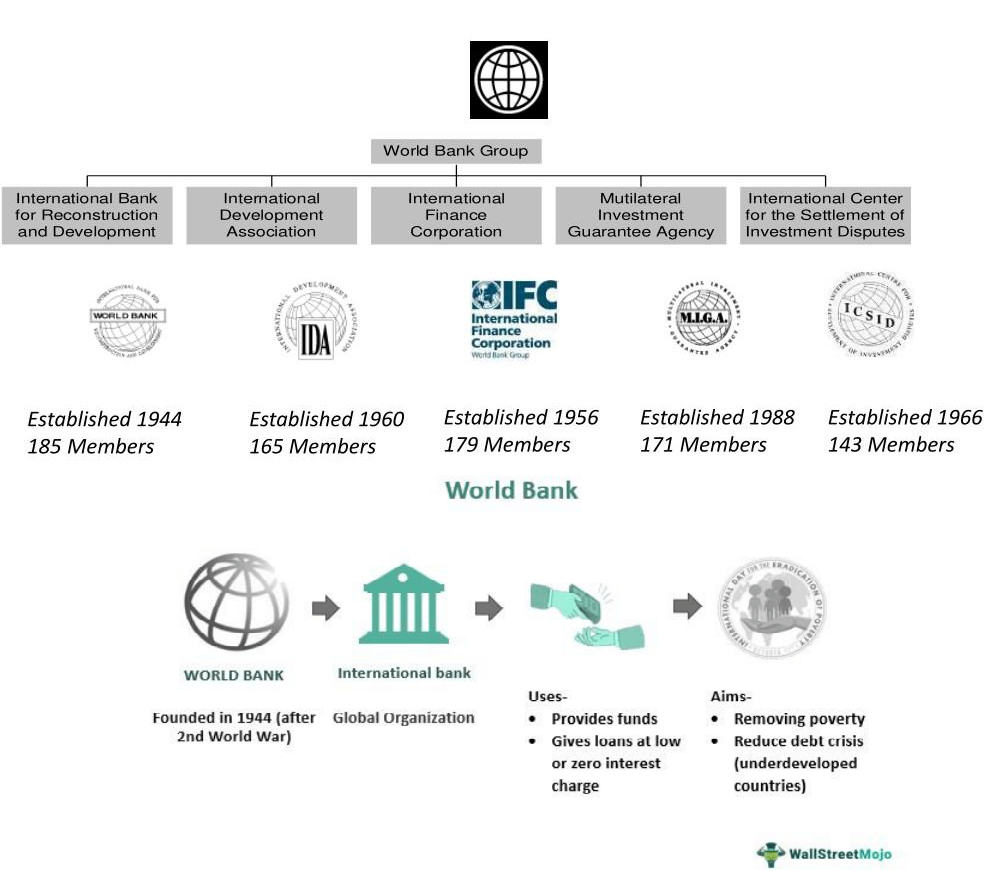
\includegraphics[scale=0.4]{WBStr.png}
    \end{figure}
\end{frame}

\begin{frame}{2.Описание данных. Всемирный Банк}
\begin{figure} \label{hompic}
            \centering
            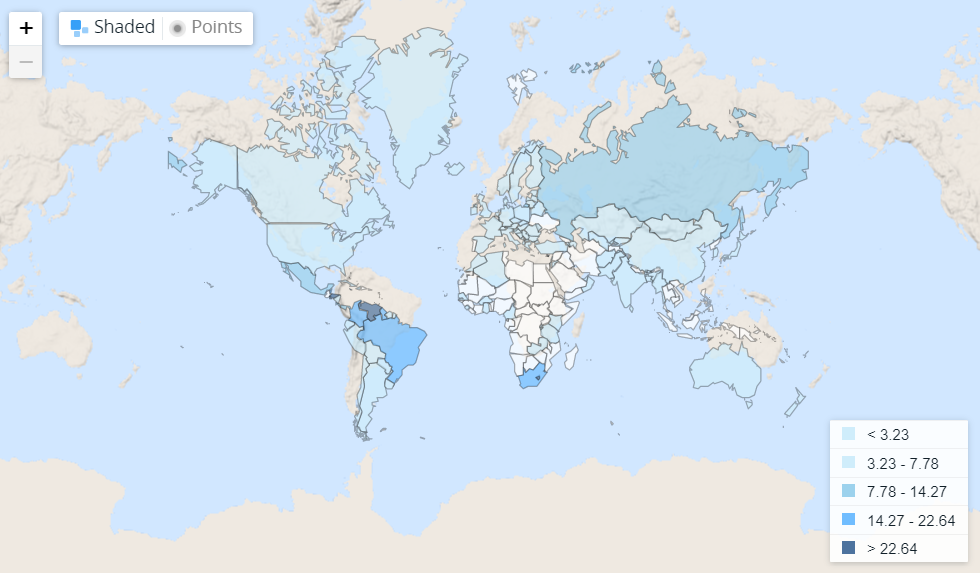
\includegraphics[scale=0.3]{homicides.png}
            \caption{Рис 2.1. Число убийств на 100000 человек за 2015 год --- данные Всемирного Банка).}
            
        \end{figure}
\end{frame}

\begin{frame}{2.Описание данных. Всемирный Банк}
\begin{figure} \label{hompic}
            \centering
            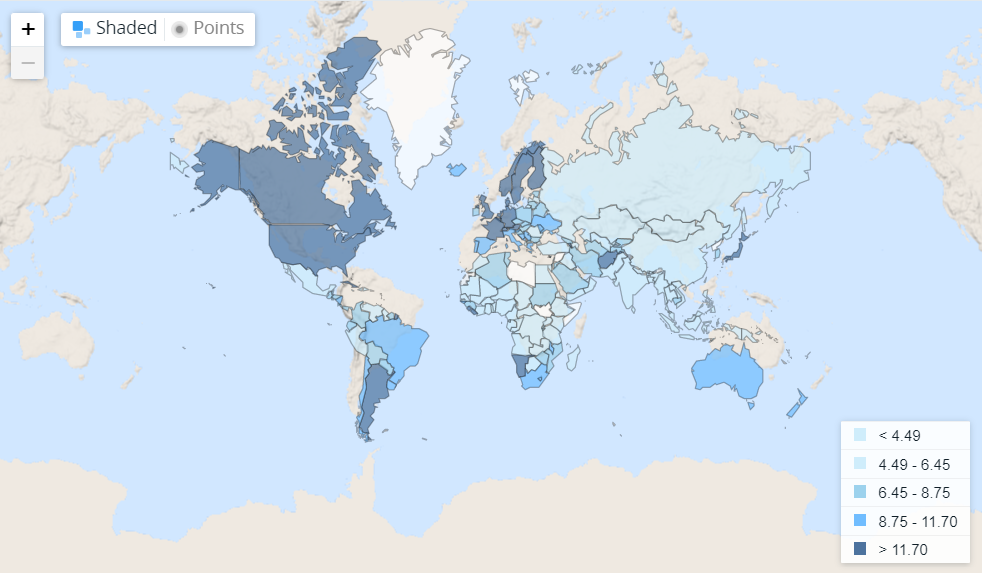
\includegraphics[scale=0.3]{medicine.png}
            \caption{Рис 2.2. Государственные расходы на медицину в процентах от ВВП  за 2015 год --- данные Всемирного Банка).}
            
        \end{figure}
\end{frame}

\begin{frame}{2.Описание данных. Всемирный Банк}
\begin{figure} \label{hompic}
            \centering
            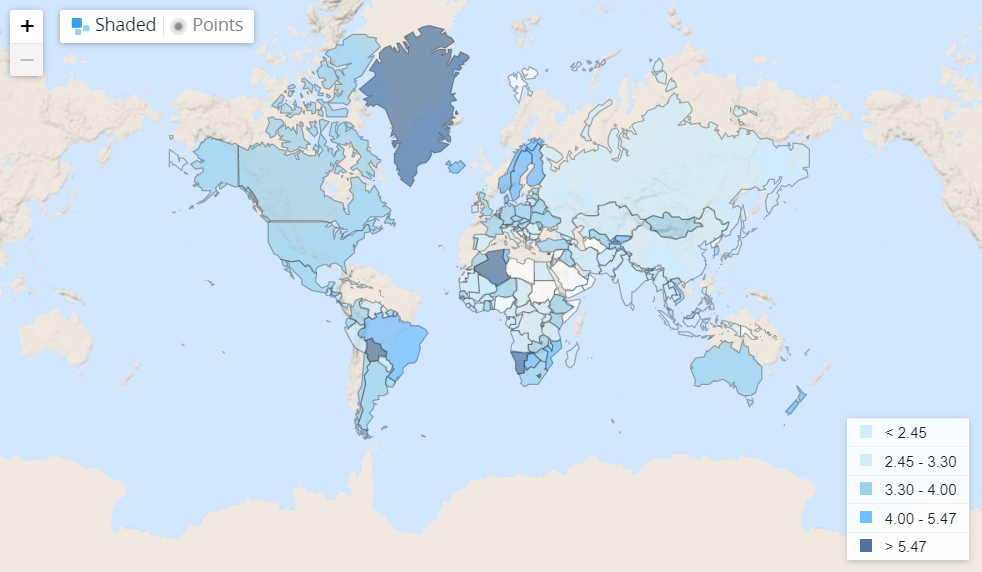
\includegraphics[scale=0.3]{education.png}
            \caption{Рис 2.3. Государственные расходы на образование в процентах от ВВП за 2015 год --- данные Всемирного Банка).}
            
        \end{figure}
\end{frame}



\begin{frame}{2.Описание данных. World Happiness Report}
Всемирный доклад о счастье  — ежегодный доклад, публикуемый подразделением ООН по поиску решений стабильного развития (UN Sustainable Development Solutions Network). В июле 2011 года Генеральная Ассамблея ООН приняла резолюцию, призывающую страны — члены ООН, оценивать счастье своего народа и использовать его как ориентир в политике государства. 

\begin{figure} \label{hompic}
            \centering
            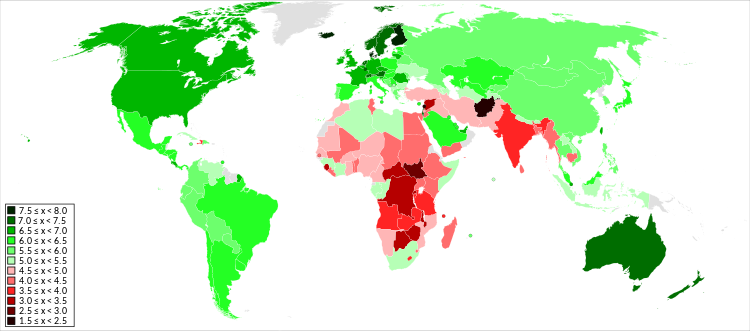
\includegraphics[scale=0.4]{Union5.png}
    \end{figure}

\end{frame}

\begin{frame}{2.Описание данных. World Happiness Report}
 

\begin{figure} \label{hompic}
            \centering
            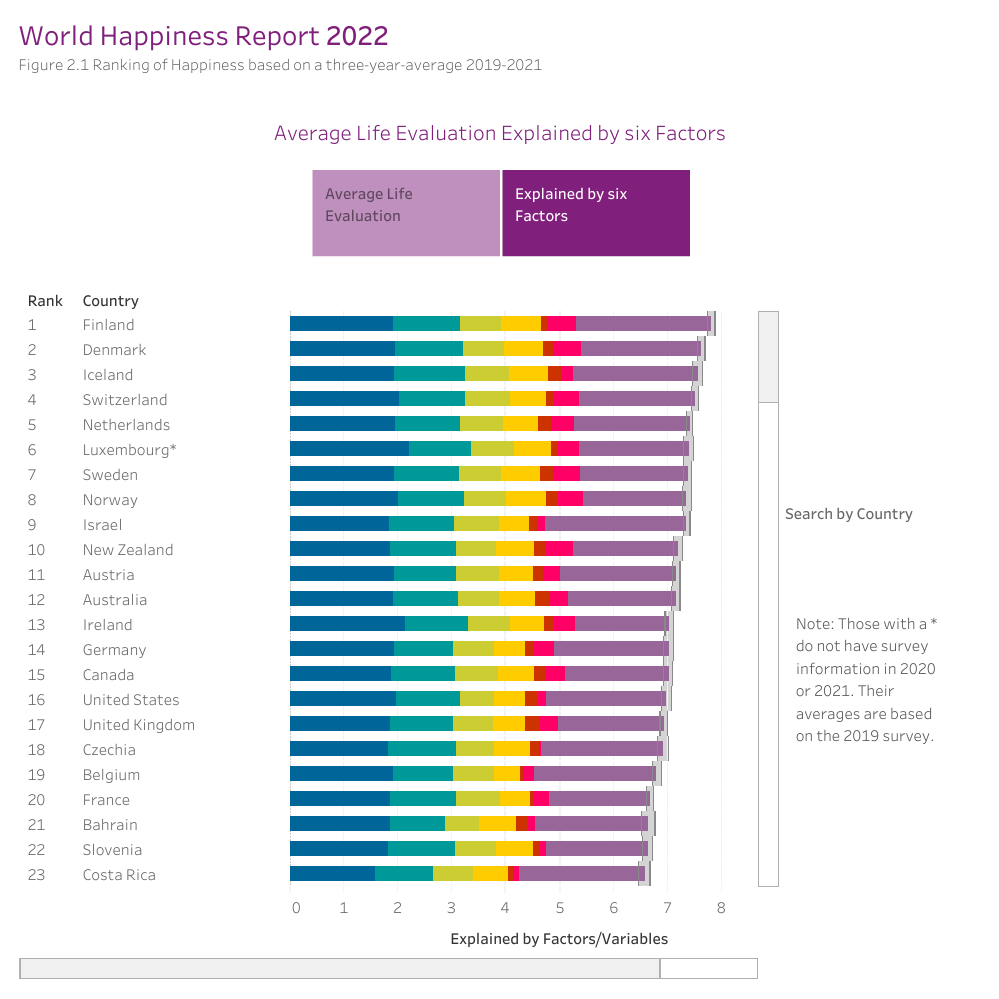
\includegraphics[scale=0.35]{FigureHappy1.png}
    \end{figure}

\end{frame}




\begin{frame}{3.Описание данных. Почему именно такие данные? Инфляция}

\begin{figure} \label{hompic}
            \centering
            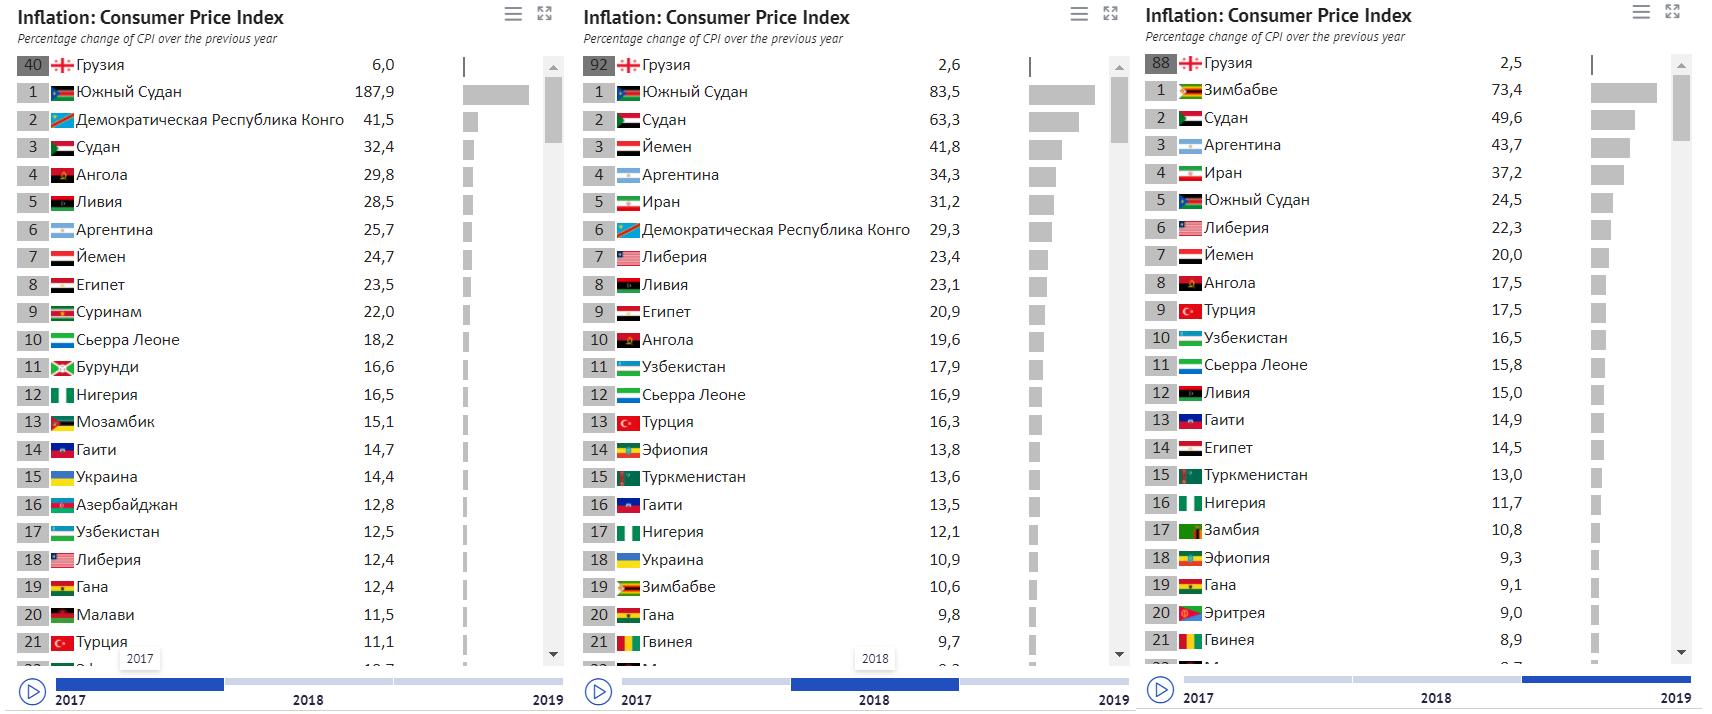
\includegraphics[scale=0.4]{Inflation.png}
    \end{figure}
    
\end{frame}

\begin{frame}{3.Описание данных. Почему именно такие данные? Безработица}

\begin{figure} \label{hompic}
            \centering
            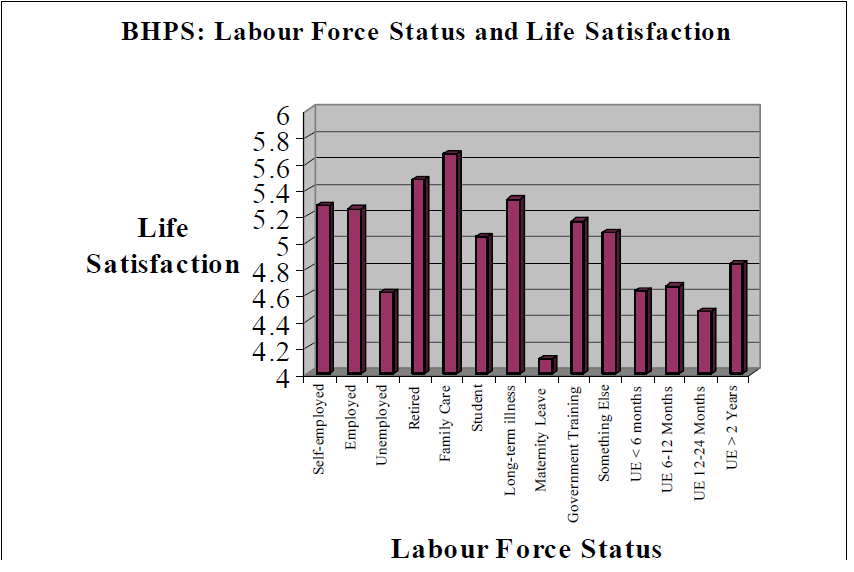
\includegraphics[scale=0.6]{2023-05-02 (5).png}
    \end{figure}
    
\end{frame}

\begin{frame}{3.Описание данных}

\begin{figure} \label{hompic}
            \centering
            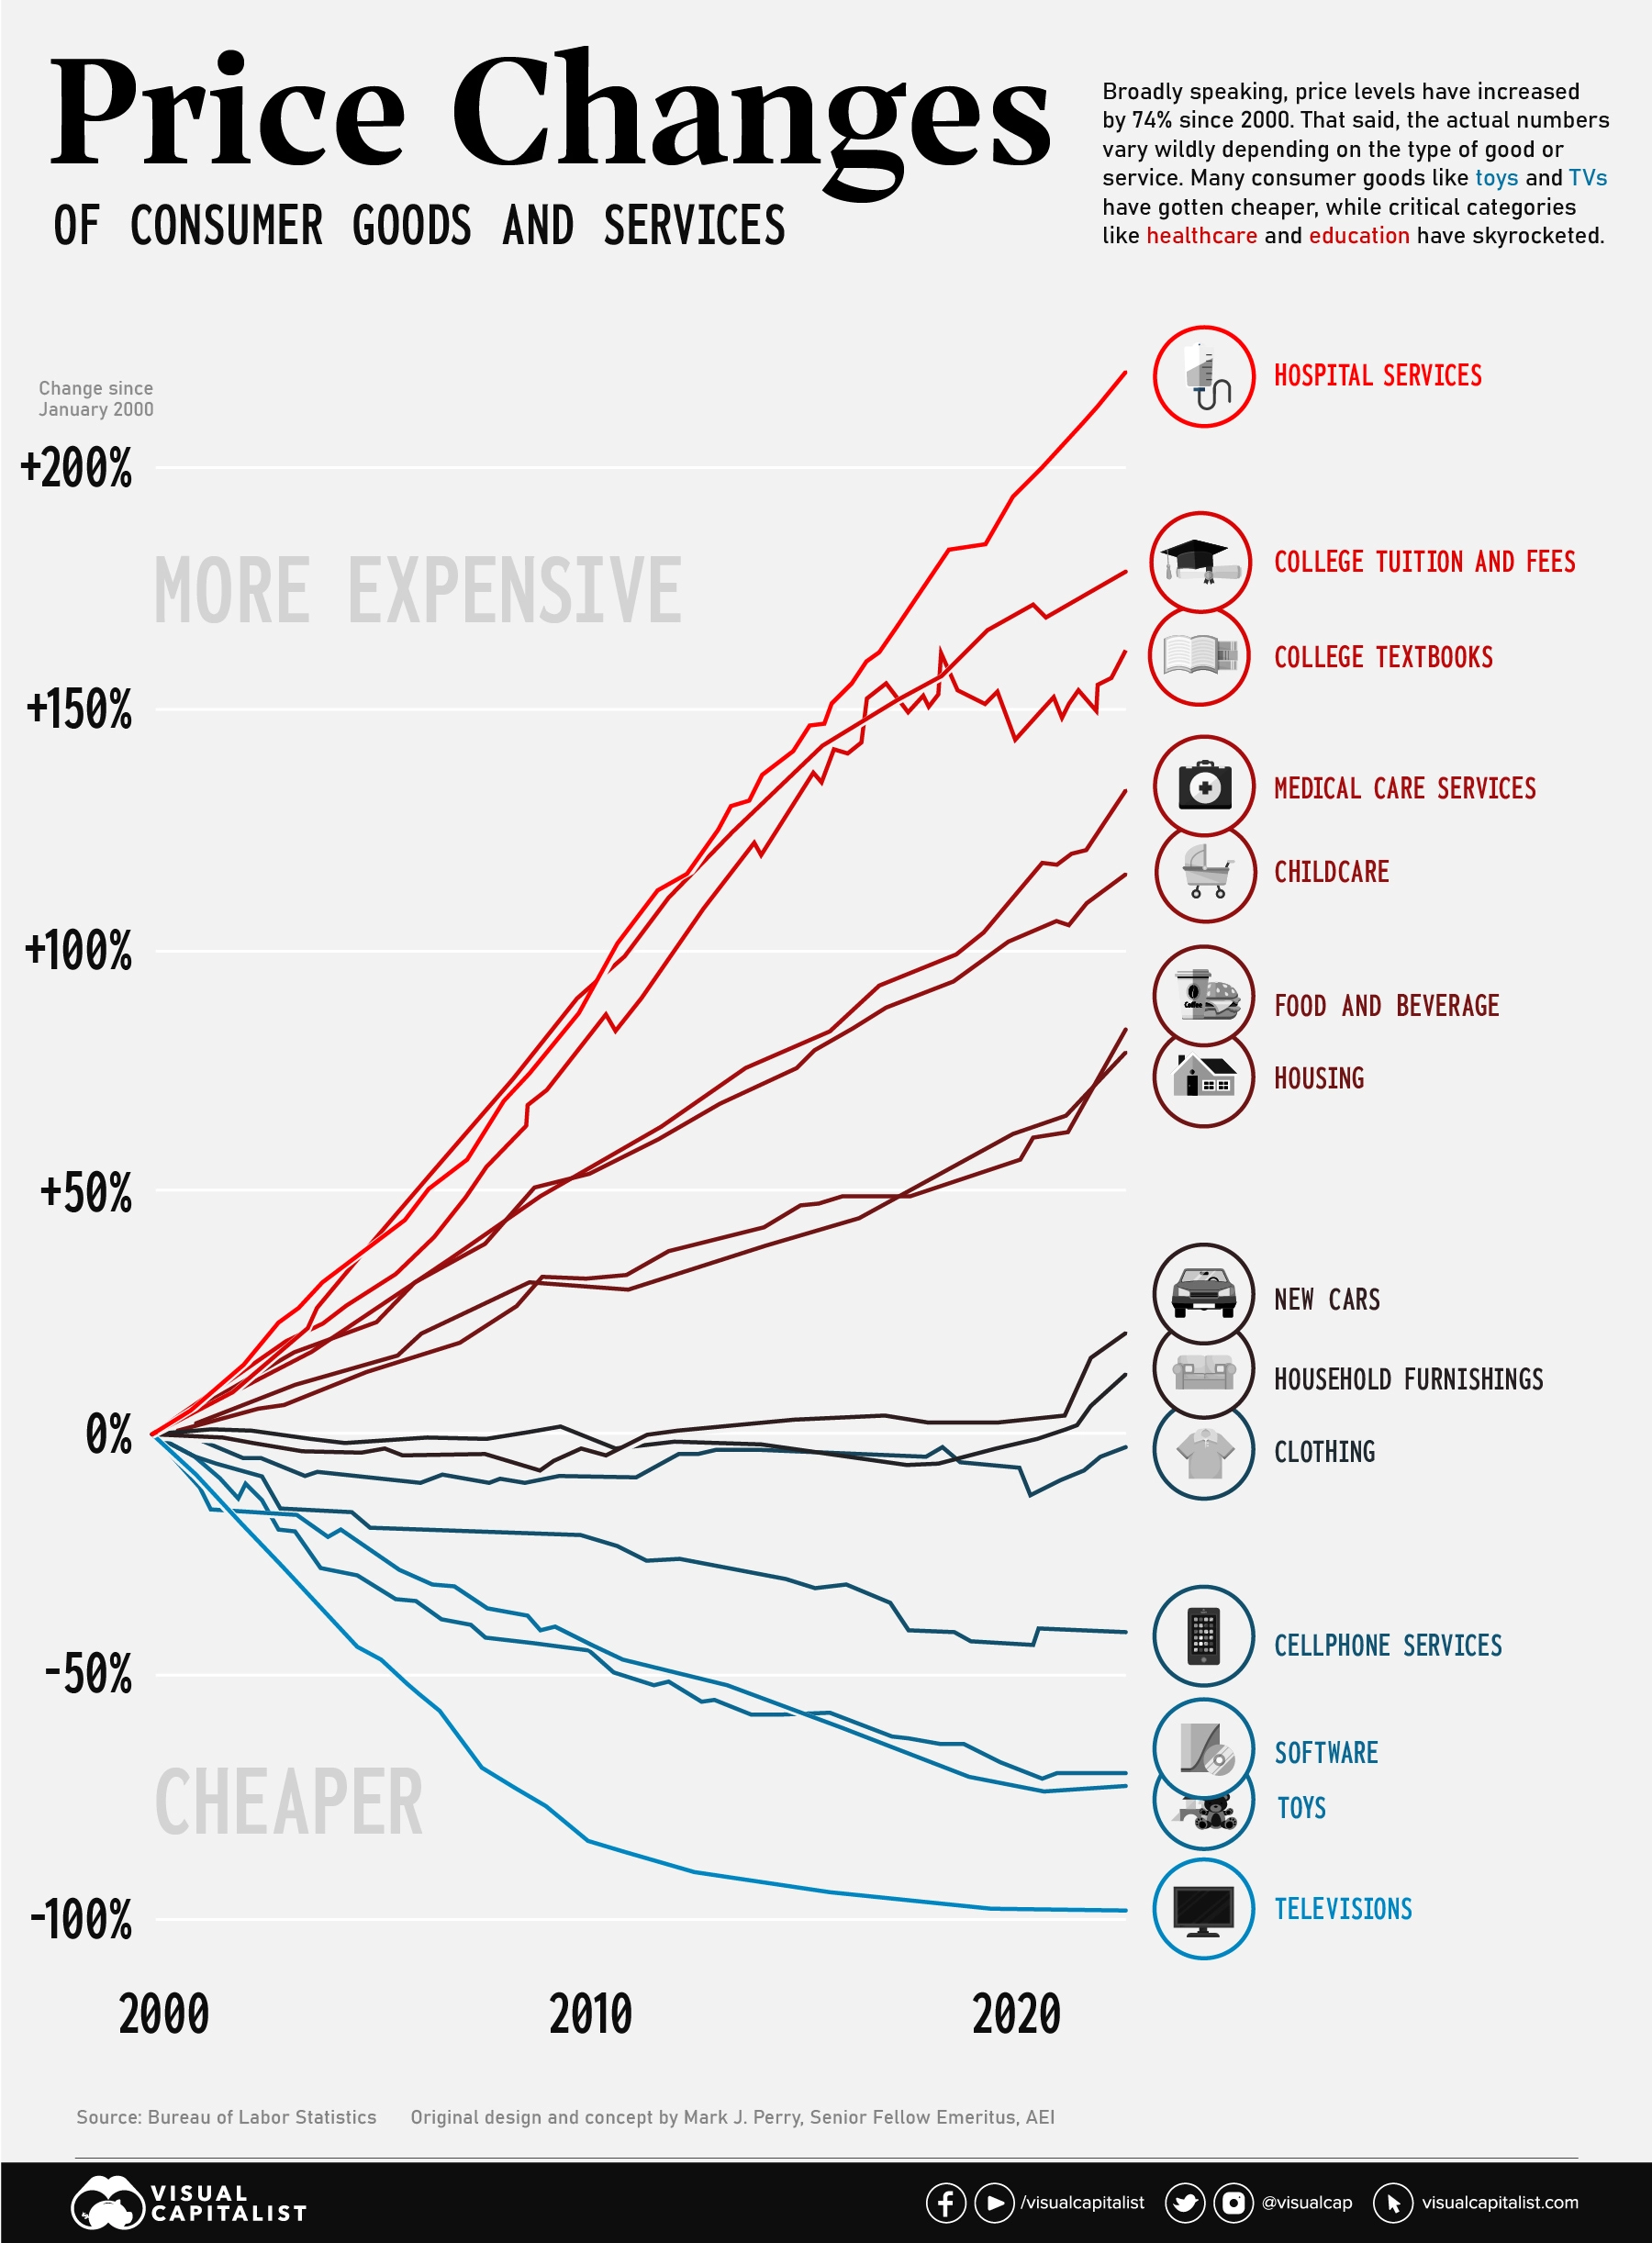
\includegraphics[scale=0.15]{price-changes-goods-services.png}
    \end{figure}
    
\end{frame}


\begin{frame}{4.Модель с ’классическими’ объясняющими переменными}
   Целевой параметр описывается уравнением:
   \footnotesize{
        \begin{align*}
         Happiness = \beta_0 + \beta_1 \lg{GDP} + \beta_2 Unemployment + \beta_3 Tax + \beta_4 Inflation + \beta_5 Medicine + \beta_6 Education.
        \end{align*}
        }
    \normalsize
    Здесь $\lg{GDP}$ --- логарифм ВВП по ППС; $Unemployment $ --- уровень безработицы; $Tax $ -- налоговая нагрузка физических лиц. $Inflation $ --- инфляция; $Medicine $ --- государственные расходы на медицину; $Education $ --- государственные расходы на образование .
\hfill \break
\hfill \break
    Эта модель построена исходя из "рекомендаций" других статей. К тому же, каждую из переменных принято ассоциировать со счастьем, насчёт каждой из переменных проводились отдельные исследования.

\end{frame}

\begin{frame}{5.Модель со ’всеми’ переменными}
   Целевой параметр описывается уравнением:
   \footnotesize
        \begin{align*}
        Happiness = \beta_0 + \beta_1 \lg{GDP} + \beta_2 Unemployment + \beta_3 Tax + \beta_4 Inflation + \beta_5 Medicine + \beta_6 Education \\
            + \beta_7 Military + \beta_8 Savings + \beta_{9} AgeRatio + \beta_{10} Homicides + \beta_{11} Fertility.
        \end{align*}
    \normalsize

    Здесь $\lg{GDP}$ --- логарифм ВВП по ППС; $Unemployment$ --- уровень безработицы; $Tax$ -- налоговая нагрузка физических лиц. $Inflation$ --- инфляция; $Medicine$ --- государственные расходы на медицину; $Education$ --- государственные расходы на образование; $Military$ --- государственные военные расходы; $Savings$ --- валовая экономия; $Patents$ --- число зарегистрированных патентов по отношению к населению государства; $AgeRatio$ --- демографическая нагрузка; $Homicides$ --- число убийств на тысячу человек .
\hfill \break
\hfill \break
    В этой версии модели мы попытались рассмотреть как можно более разнообразные метрики благополучия страны.

\end{frame}

\begin{frame}{6.Результаты и их интерпретация}
   \begin{figure} \label{hompic}
            \centering
            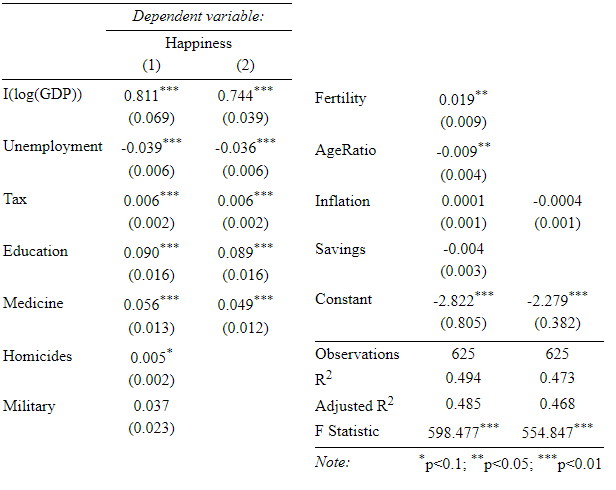
\includegraphics[scale=0.75]{UnionTable.png}
    \end{figure}

\end{frame}




\begin{frame}{7.Выводы}
   \small
   В статье исследуются две модели, описывающие зависимость счастья от некоторых макроэкономических показателей. Исследования подобных моделей помогают искать ответ на вопрос об этой связи и, на основании этого, строить рекомендации по осуществлению государственной политики и подтверждать (или опровергать) общепринятые идеи.
        \\
        Из ключевых результатов работы можно выделить следующее:
        \begin{itemize}
            \item Общепринятые и очевидные факты: экономическое развитие страны и увеличение доли бюджетных трат на образование значимо повышают уровень счастья граждан, увеличение же безработицы его уменьшает --- были подтверждены. Кроме того, были даны ссылки на публикации, более подробно исследующие эти темы.
            \item Увеличение налогов значимо повышает уровень счастья в модели.
            \item Не было выявлено значимого влияния инфляции, доли военных трат и демографической нагрузки на счастье.
            \item Не было выявлено значимого влияния числа убийств на счастье. Впрочем, похоже, что это свидетельствует о несостоятельности этой метрики, а не об отсутствии подобной связи.
        \end{itemize}
        

    \normalsize


\end{frame}

 \begin{frame}{8.Ссылки}
\tiny
 \begin{thebibliography}{100}
\bibitem{} \label{Easterlin}
            Easterlin R. A.
            Does Economic Growth Improve the Human Lot? Some Empirical Evidence.
            --- \textit{Nations and Households in Economic Growth}, 
            89-125, 1974.

            \bibitem{} \label{KahnemanDeaton}
            Kahneman D., Deaton A. 
            High income improves evaluation of life but not emotional well-being. 
            --- \textit{Proc Natl Acad Sci USA},
            \textbf{38}, 2010.

            \bibitem{} \label{DiTella}
            Di Tella R., MacCulloch R. J., Oswald A. J.
            The macroeconomics of happiness. 
           --- \textit{Review of Economics and Statistics}, 
            \textbf{85}, 1999. 

            \bibitem{} \label{Easterlin2}
            Easterlin R. A.
            Will Raising the Incomes of All Increase the Happiness of All?
            --- \textit{Journal of Economic Behaviour and Organization},
            \textbf{27}, 35-48, 1999. 

            \bibitem{} \label{Clark}
            Clark A. E., Oswald A. J.
            Unhappiness and Unemployment.
            --- \textit{Economic Journal}, 
            \textbf{104}, 648-659, 1994. 

            \bibitem{} \label{Winkelmann}
            Winkelmann L, Winkelmann R.
            Why are the unemployed so unhappy?
            --- \textit{Economica}, 
            \textbf{65}, 1-15, 1998. 

            \bibitem{} \label{tax}
            Hutchinson T., Ahmed I., Buryi P.
            Impact of income tax on happiness: evidence from the United States. 
            --- \textit{Applied Economics Letters}, 1-3.
            1-3, 2016.

            \bibitem{} \label{Clarkunemp}
            Clark A. E.
            A Note on Unhappiness and Unemployment Duration.
            --- \textit{IZA Discussion Paper No. 2406}, 
            2006. 
            
            \bibitem{} \label{Inflation}
            Shiller J. R.
            Why Do People Dislike Inflation?
            --- \textit{NBER Working Paper}, 
            \textbf{5539}, 1996. 

            \bibitem{} \label{medicine}
            Dfarhud D., Maryam M., Khanahmadi M. 
            Happiness & Health: The Biological Factors-Systematic Review Article.
            --- \textit{Iranian Journal of Public Health}, 
            \textbf{43}, 1468-1477, 2014. 

            \bibitem{} \label{Education}
            Satoshi Araki.
            Does Education Make People Happy? Spotlighting the Overlooked Societal Condition.
            --- \textit{Journal of Happiness Studies}, 
            \textbf{23}, 587-629, 2021.
    \end{thebibliography}
 \end{frame}

 
\end{document}